\chapter{Tests, Validation et Résultats}
\label{chap:testing_validation_results}
\section{Introduction}

\par Après l'implémentation des principaux modules de l'application \textbf{TuniPark}, une phase de tests et de validation a été réalisée afin de vérifier le bon fonctionnement des fonctionnalités développées. Cette étape avait pour objectif de s'assurer que l'application mobile, la plateforme web d'administration, les services Backend ainsi que les différents services externes fonctionnaient correctement de manière intégrée.

\par Ce chapitre présente la stratégie de test adoptée durant le développement, les outils utilisés pour la validation des API et des fonctionnalités, les principaux scénarios testés ainsi que les résultats obtenus. Il met également en évidence les difficultés rencontrées au cours de la phase de validation.

\section{Stratégie de test}

\par Les tests ont été réalisés progressivement tout au long du développement de l'application. Chaque fonctionnalité a été validée individuellement avant d'être testée après son intégration avec les autres modules. Cette approche a permis d'identifier rapidement les anomalies et de garantir le bon fonctionnement global de la plateforme.

\par La validation a principalement porté sur les fonctionnalités essentielles de TuniPark, notamment l'authentification des utilisateurs, la gestion des parkings, la création des sessions de stationnement, les paiements électroniques, les notifications Push ainsi que le système de recommandation intelligent.

\par Les principaux objectifs de cette phase de validation étaient les suivants :

\begin{itemize}
\item vérifier le bon fonctionnement de l'authentification et du contrôle d'accès ;
\item valider les opérations de gestion des parkings ;
\item confirmer le bon déroulement de la création et du paiement des sessions de stationnement ;
\item vérifier l'envoi des notifications Push ;
\item valider le fonctionnement du système de recommandation intelligent ;
\item s'assurer de la bonne communication entre les différents services de la plateforme.
\end{itemize}
\section{Outil de test des API}

\par Durant la phase de validation du Backend, l'interface \textbf{Swagger} intégrée à \textbf{NestJS} a été utilisée afin de tester directement les API développées. Cet outil a permis d'envoyer des requêtes HTTP, d'analyser les réponses du serveur et de vérifier le bon fonctionnement des différents points d'accès sans passer systématiquement par l'application mobile.

\par Dans le cadre de ce projet, Swagger \cite{swagger} a été utilisé pour tester les principales fonctionnalités de l'application, notamment l'authentification, la gestion des utilisateurs, des parkings, des sessions de stationnement, des paiements, des notifications ainsi que les routes protégées nécessitant un jeton JWT. Il a également permis de vérifier les paramètres des requêtes, les réponses retournées par le serveur ainsi que les différents codes de statut HTTP.

\begin{figure}[H]
    \centering
    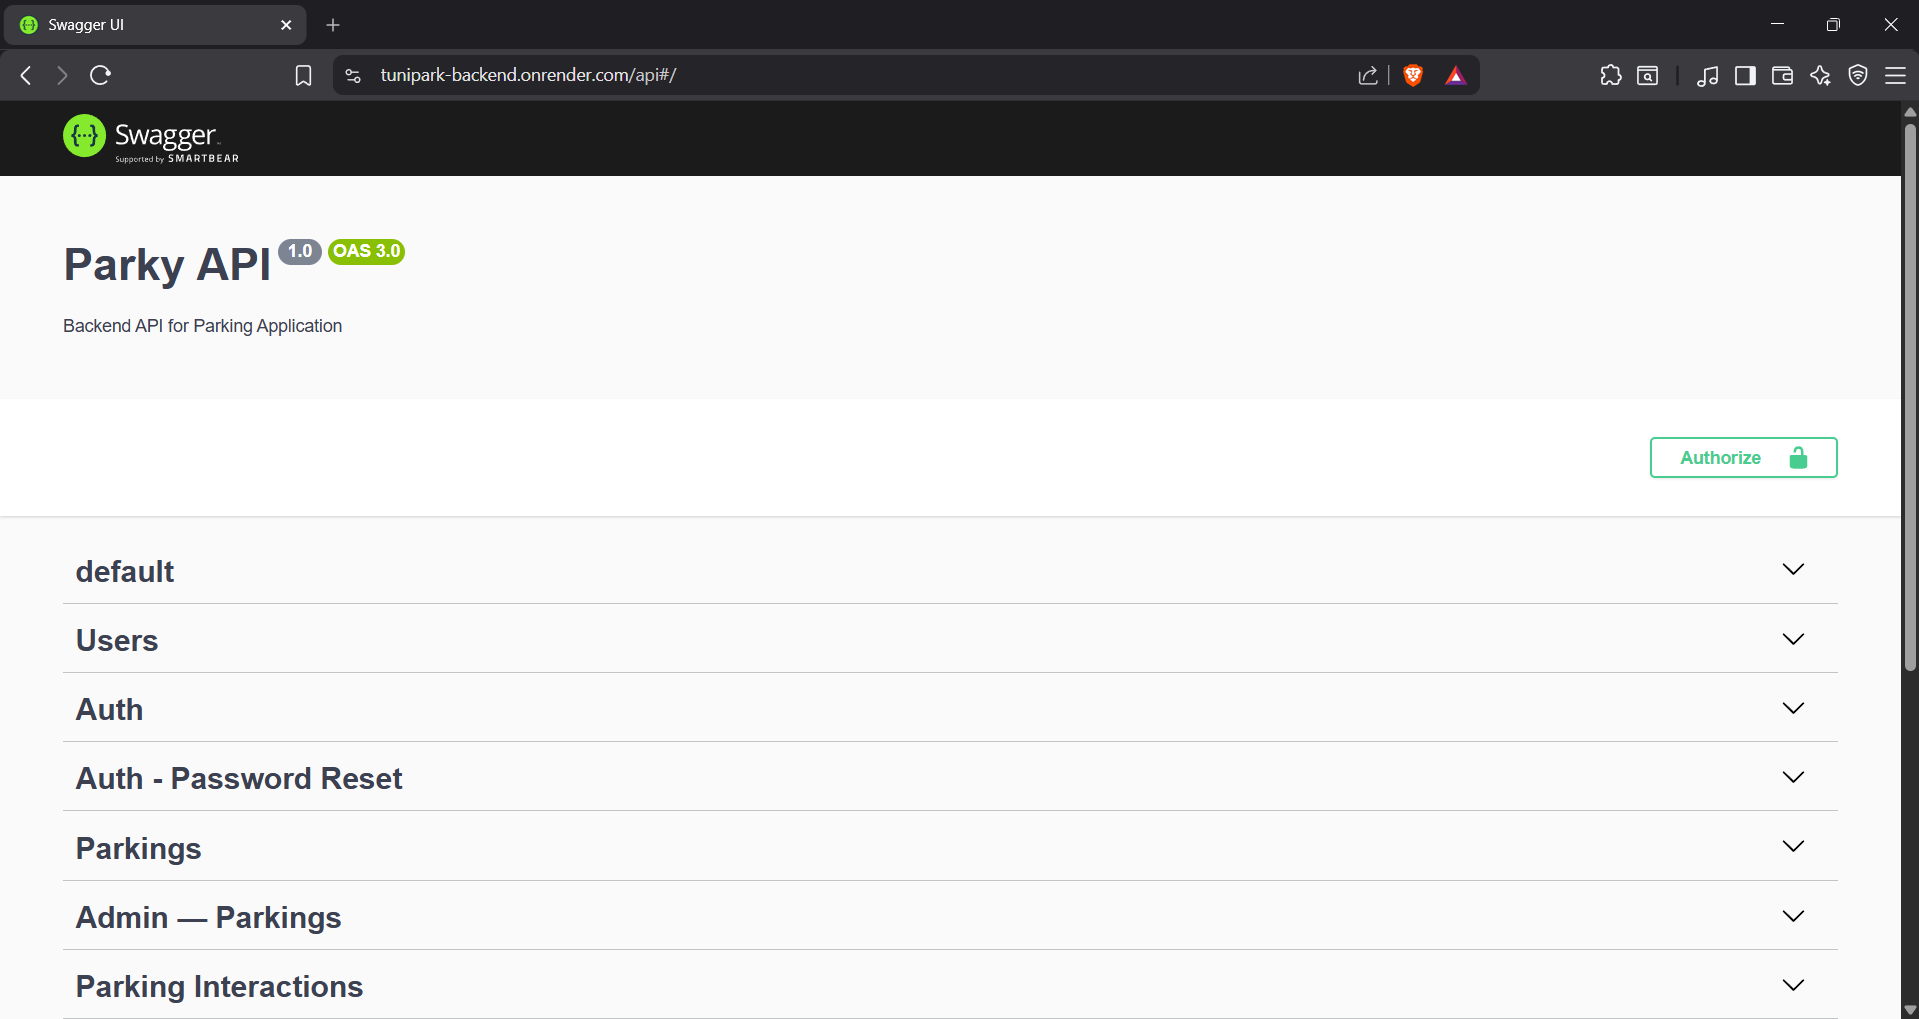
\includegraphics[width=0.9\textwidth]{img/swagger.png}
    \caption{Documentation et tests des API à l'aide de Swagger}
    \label{fig:swagger}
\end{figure}
\section{Validation des API du Backend}

\par La validation des API a débuté par le test du point d'accès d'authentification. Après une connexion réussie, le Backend génère un \textit{Access Token} ainsi qu'un \textit{Refresh Token}. Ces jetons sont ensuite utilisés pour accéder aux différentes routes sécurisées de l'application et vérifier le contrôle d'accès selon les rôles des utilisateurs.

\begin{figure}[H]
    \centering
    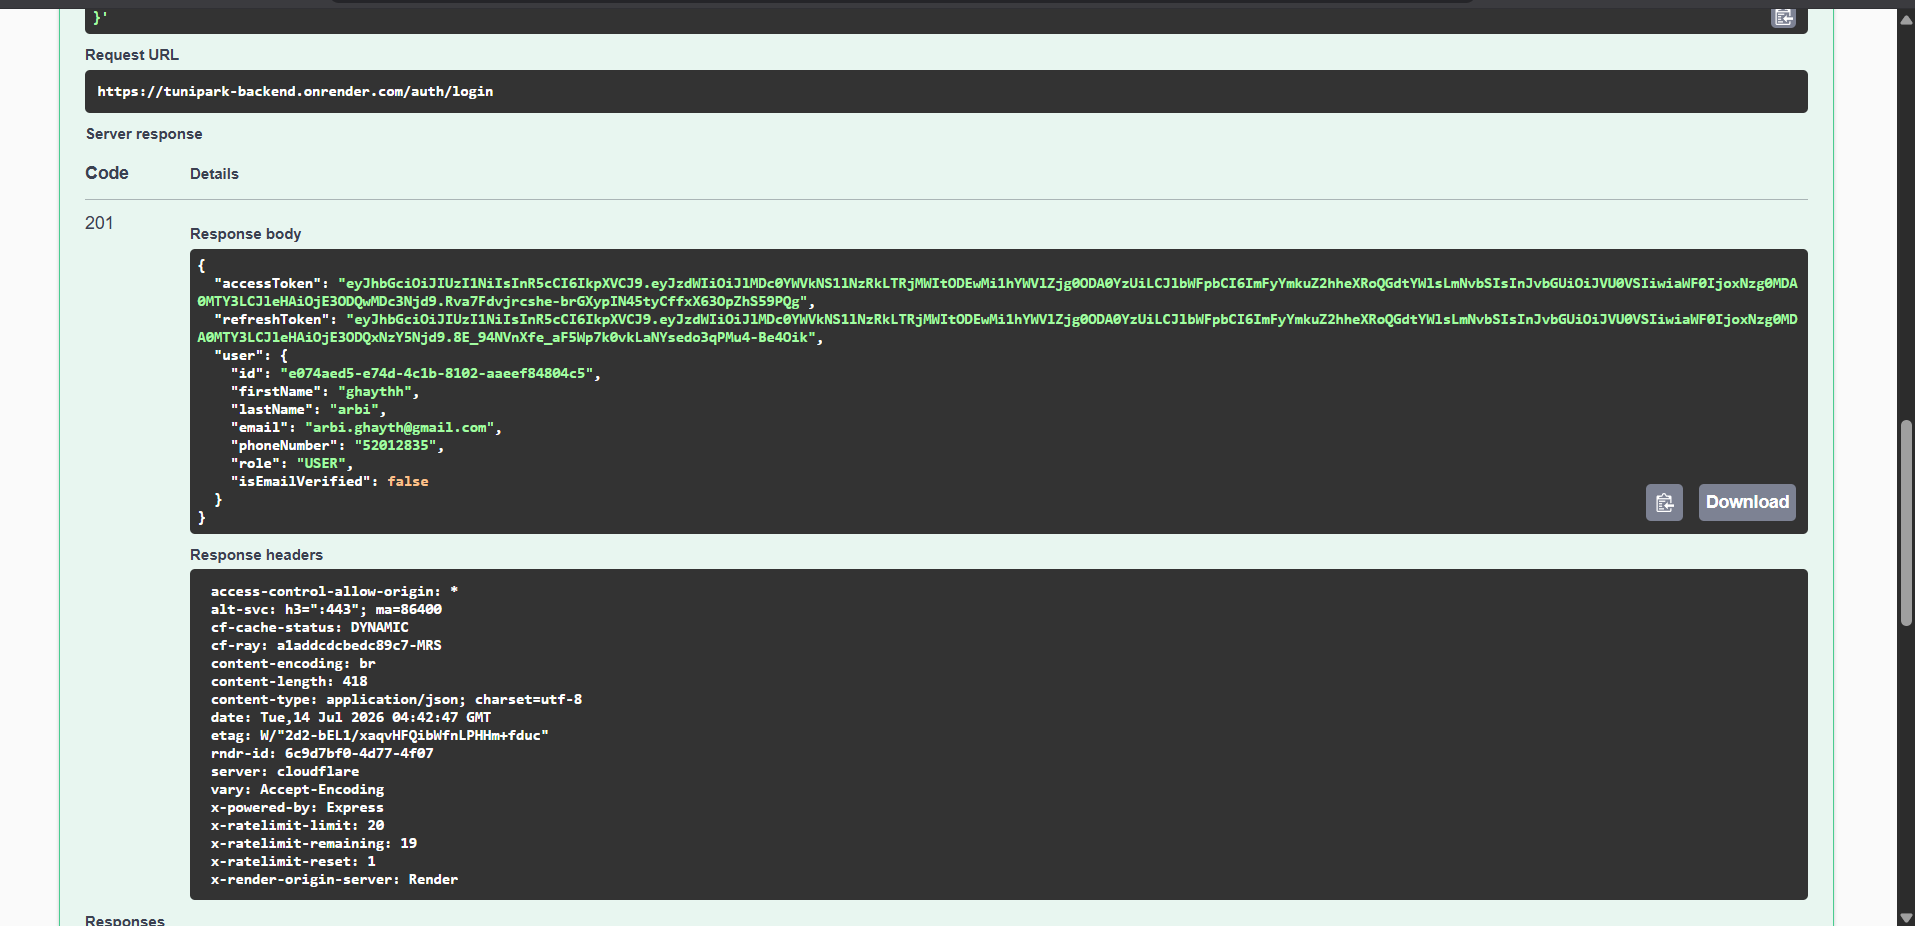
\includegraphics[width=0.95\textwidth]{img/swagger_login.png}
    \caption{Validation de l'API d'authentification avec Swagger}
    \label{fig:swagger_login_test}
\end{figure}

\par Des tests complémentaires ont ensuite été réalisés sur les principales API de l'application, notamment la gestion des parkings, la création et le paiement des sessions de stationnement, les notifications, le système de recommandation ainsi que les opérations d'administration. Ces essais ont confirmé que les requêtes valides étaient correctement traitées et que le Backend retournait les réponses ainsi que les codes d'erreur appropriés lorsque les données fournies étaient incomplètes ou invalides.

\section{Tests fonctionnels}

\par Les tests fonctionnels ont été réalisés afin de vérifier le bon fonctionnement de l'application \textbf{TuniPark} du point de vue des utilisateurs et des administrateurs. Chaque fonctionnalité a été testée dans des conditions d'utilisation réelles afin de s'assurer que les résultats obtenus correspondaient au comportement attendu.

\par Les essais ont porté sur les principales fonctionnalités de l'application, notamment l'authentification, la gestion des parkings, la création des sessions de stationnement, les paiements électroniques, les notifications Push ainsi que le système de recommandation intelligent. Les résultats obtenus ont permis de confirmer le bon fonctionnement de l'ensemble des modules développés.

\subsection{Tests d'authentification et de contrôle d'accès}

\par Les tests d'authentification ont permis de vérifier la connexion des utilisateurs, la génération des jetons JWT ainsi que le contrôle d'accès aux ressources protégées. Le mécanisme de renouvellement automatique des jetons à l'aide du \textit{Refresh Token} a également été validé.

\begin{table}[H]
\centering
\small
\renewcommand{\arraystretch}{1.25}
\begin{tabular}{|p{0.35\textwidth}|p{0.38\textwidth}|p{0.17\textwidth}|}
\hline
\textbf{Test} & \textbf{Comportement attendu} & \textbf{Résultat} \\
\hline
Connexion avec des identifiants valides & L'utilisateur accède à l'application. & Réussi \\
\hline
Connexion avec des identifiants invalides & Message d'erreur affiché. & Réussi \\
\hline
Accès sans jeton JWT & La requête est refusée. & Réussi \\
\hline
Renouvellement de l'Access Token & Un nouveau jeton est généré via le Refresh Token. & Réussi \\
\hline
\end{tabular}
\caption{Tests d'authentification et de contrôle d'accès}
\label{tab:auth_tests}
\end{table}

\subsection{Tests de gestion des parkings}

\par Les fonctionnalités de gestion des parkings ont été testées aussi bien du côté propriétaire que du côté administrateur. Les essais ont permis de vérifier la création d'un parking privé, sa validation par un administrateur ainsi que la mise à jour de ses informations.

\begin{table}[H]
\centering
\small
\renewcommand{\arraystretch}{1.25}
\begin{tabular}{|p{0.35\textwidth}|p{0.38\textwidth}|p{0.17\textwidth}|}
\hline
\textbf{Test} & \textbf{Comportement attendu} & \textbf{Résultat} \\
\hline
Ajouter un parking privé & Parking créé avec le statut \texttt{PENDING}. & Réussi \\
\hline
Valider un parking & Le statut devient \texttt{ACTIVE}. & Réussi \\
\hline
Rejeter un parking & Le parking reste indisponible. & Réussi \\
\hline
Modifier les informations d'un parking & Les modifications sont enregistrées. & Réussi \\
\hline
\end{tabular}
\caption{Tests de gestion des parkings}
\label{tab:parking_tests}
\end{table}

\subsection{Tests des sessions de stationnement et des paiements}

\par Les scénarios de création d'une session de stationnement et de paiement via Flouci ont été validés afin de vérifier le bon déroulement du processus complet.

\begin{table}[H]
\centering
\small
\renewcommand{\arraystretch}{1.25}
\begin{tabular}{|p{0.35\textwidth}|p{0.38\textwidth}|p{0.17\textwidth}|}
\hline
\textbf{Test} & \textbf{Comportement attendu} & \textbf{Résultat} \\
\hline
Créer une session & Une session est créée avec le statut \texttt{CREATED}. & Réussi \\
\hline
Paiement Flouci validé & La session passe au statut \texttt{ACTIVE}. & Réussi \\
\hline
Paiement annulé & La session n'est pas activée. & Réussi \\
\hline
Fin de session & Le paiement est enregistré correctement. & Réussi \\
\hline
\end{tabular}
\caption{Tests des sessions de stationnement et des paiements}
\label{tab:session_tests}
\end{table}

\subsection{Tests des notifications}

\par Les notifications internes ainsi que les notifications Push envoyées via Firebase Cloud Messaging ont été testées afin de vérifier leur création, leur envoi et leur affichage dans l'application.

\begin{table}[H]
\centering
\small
\renewcommand{\arraystretch}{1.25}
\begin{tabular}{|p{0.35\textwidth}|p{0.38\textwidth}|p{0.17\textwidth}|}
\hline
\textbf{Test} & \textbf{Comportement attendu} & \textbf{Résultat} \\
\hline
Créer une notification & Notification enregistrée en base de données. & Réussi \\
\hline
Notification Push FCM & Réception sur le téléphone mobile. & Réussi \\
\hline
Marquer une notification comme lue & Mise à jour du statut de lecture. & Réussi \\
\hline
\end{tabular}
\caption{Tests des notifications}
\label{tab:notification_tests}
\end{table}

\subsection{Tests du système de recommandation}

\par Le système de recommandation intelligent a été testé afin de vérifier le fonctionnement du modèle Random Forest et la génération des recommandations de parkings.

\begin{table}[H]
\centering
\small
\renewcommand{\arraystretch}{1.25}
\begin{tabular}{|p{0.35\textwidth}|p{0.38\textwidth}|p{0.17\textwidth}|}
\hline
\textbf{Test} & \textbf{Comportement attendu} & \textbf{Résultat} \\
\hline
Demande de recommandations & Liste des parkings recommandés affichée. & Réussi \\
\hline
Microservice IA disponible & Calcul des scores avec Random Forest. & Réussi \\
\hline
Indisponibilité du microservice & Utilisation de l'algorithme de secours. & Réussi \\
\hline
\end{tabular}
\caption{Tests du système de recommandation}
\label{tab:ai_tests}
\end{table}


\section{Validation de la base de données}

\par La validation de la base de données \textbf{PostgreSQL} a été réalisée en vérifiant que les différentes opérations effectuées depuis l'application entraînaient bien les modifications attendues au niveau des données. Les résultats obtenus ont été contrôlés à travers les réponses des API ainsi que les journaux d'exécution du Backend.

\par Les contrôles ont principalement concerné la mise en place des comptes utilisateurs, l'intégration et l'approbation des parkings, l'établissement des sessions de stationnement, le suivi des paiements, les alertes, ainsi que les communications employées par le système de recommandation. Les différents tests ont confirmé que les opérations de création, de modification et de suppression étaient correctement prises en compte et que la cohérence entre les entités associées était bien préservée.
\begin{figure}[H]
    \centering
    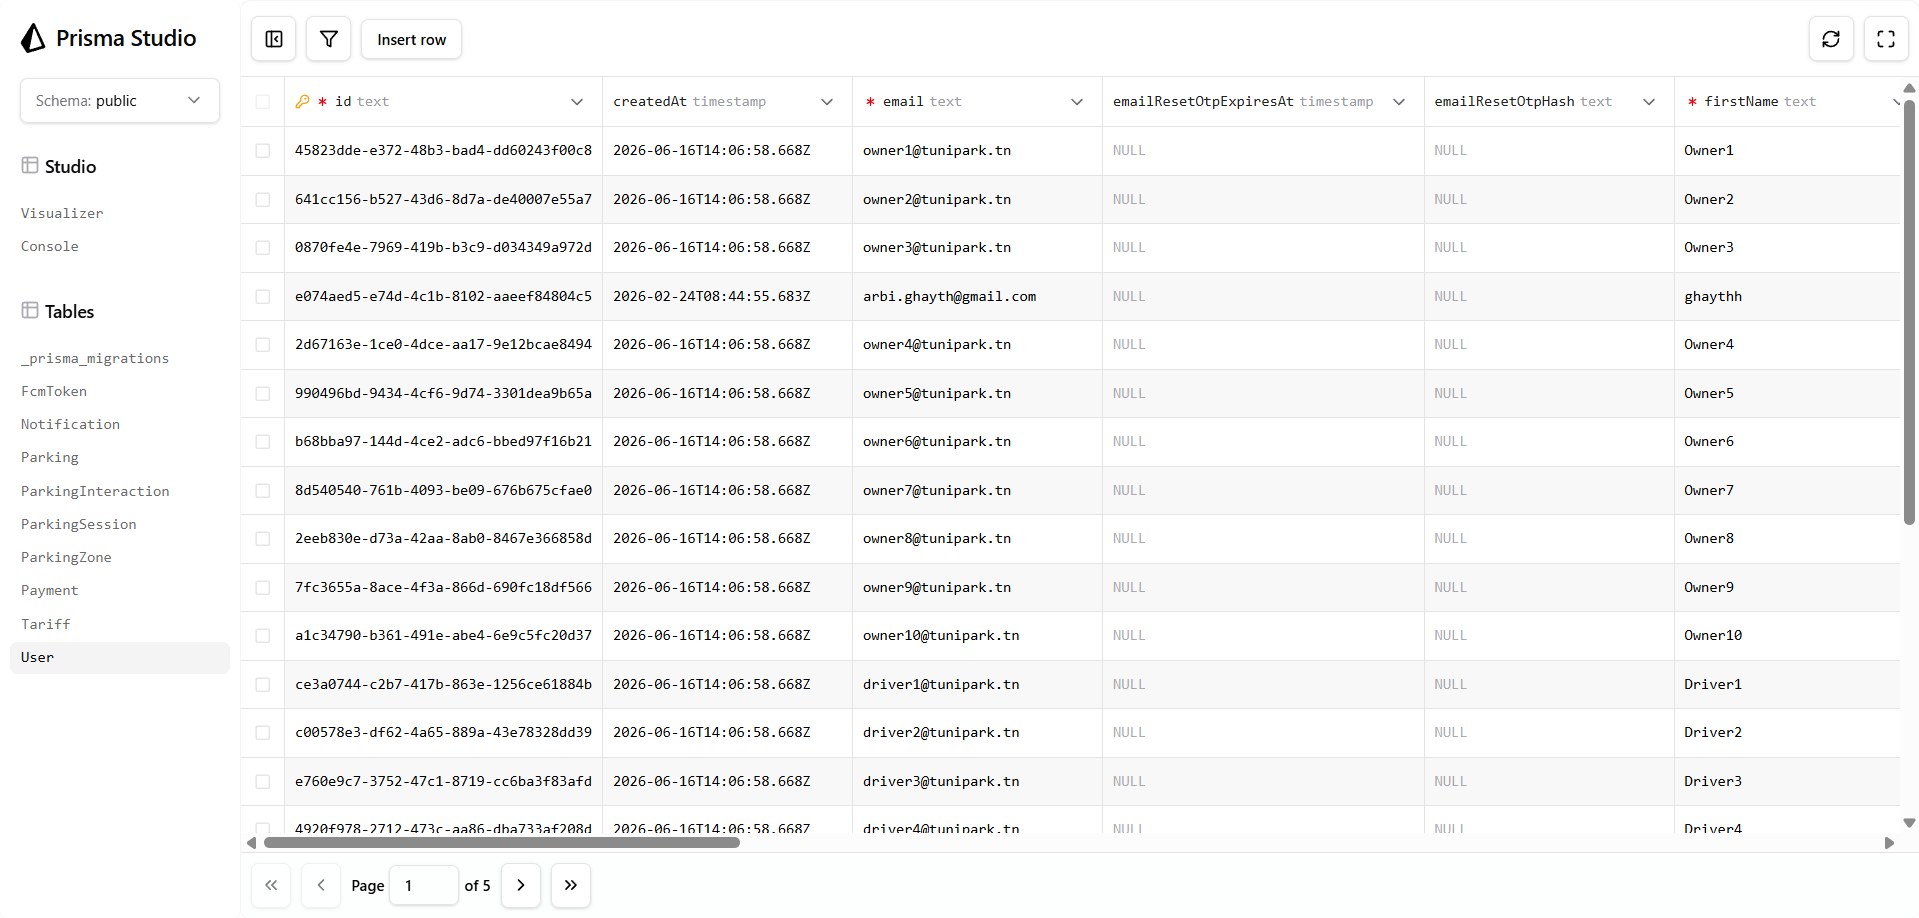
\includegraphics[width=0.95\textwidth]{img/postgresql_validation.png}
    \caption{Validation des données enregistrées dans PostgreSQL}
    \label{fig:postgres_validation}
\end{figure}


\section{Validation des services externes}

\par Plusieurs fonctionnalités de l'application \textbf{TuniPark} reposent sur des services externes. Des tests ont donc été réalisés afin de vérifier leur bonne intégration avec le Backend. Les validations ont principalement concerné le paiement électronique avec \textbf{Flouci}, l'envoi des notifications Push via \textbf{Firebase Cloud Messaging} ainsi que le stockage des images sur \textbf{Cloudinary}.

\subsection{Validation des paiements avec Flouci}

\par L'intégration de Flouci a été validée lors de la création d'une session de stationnement. Après la sélection d'un parking, l'utilisateur a été redirigé vers la plateforme de paiement. Une fois la transaction confirmée, Flouci a transmis le résultat au Backend, qui a mis à jour le statut du paiement ainsi que celui de la session de stationnement.

\begin{figure}[H]
    \centering
    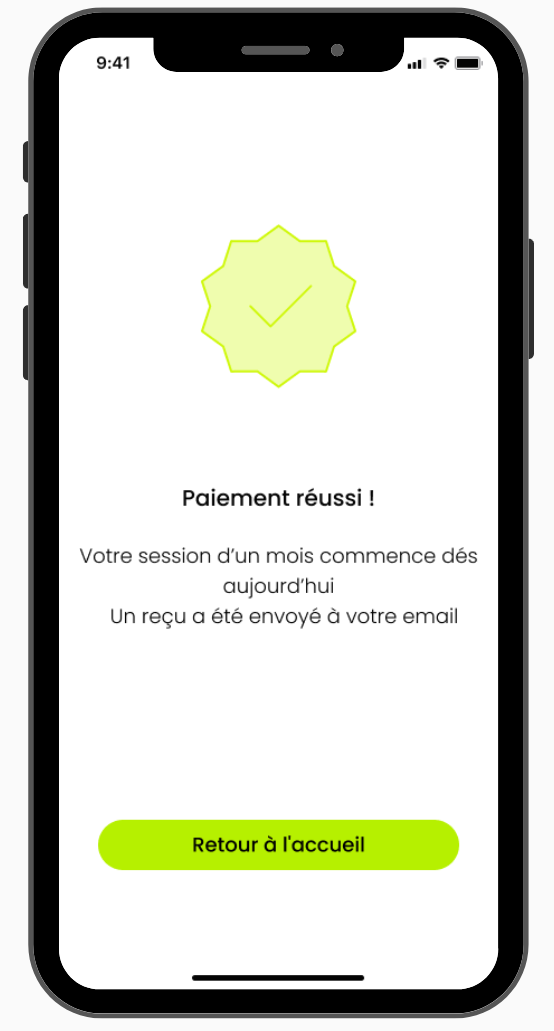
\includegraphics[width=0.5\textwidth]{img/flouci_test.png}
    \caption{Validation d'un paiement avec Flouci}
    \label{fig:flouci_test}
\end{figure}

\par Les essais réalisés ont confirmé le bon fonctionnement du processus de paiement et la mise à jour correcte des informations enregistrées dans la base de données.

\subsection{Validation des notifications Firebase}

\par Les notifications Push ont été testées à l'aide de Firebase Cloud Messaging. Lorsqu'un événement nécessitant une notification se produit, le Backend récupère le jeton FCM de l'utilisateur et transmet la notification au service Firebase, qui l'envoie ensuite vers l'appareil mobile.

\begin{figure}[H]
    \centering
    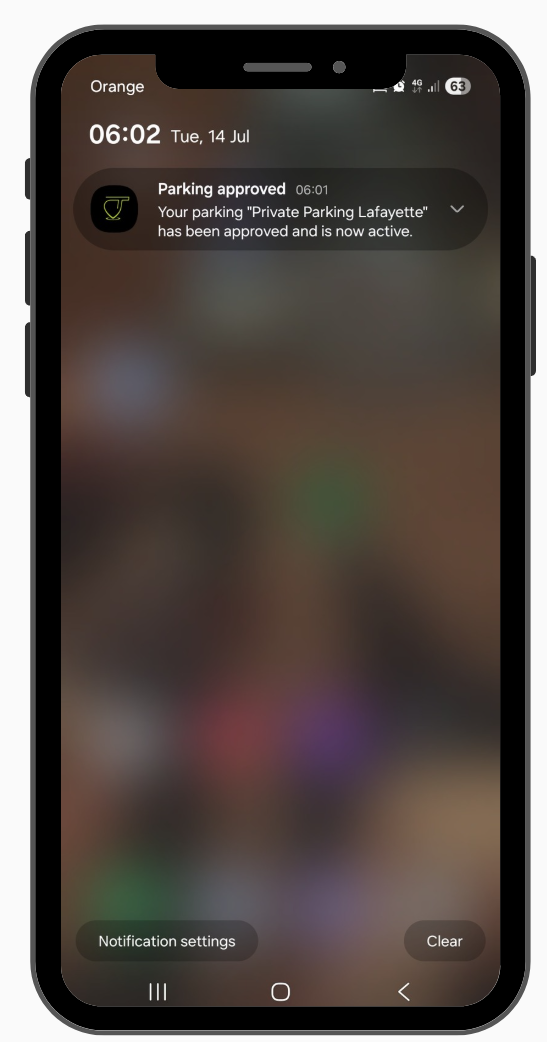
\includegraphics[width=0.45\textwidth]{img/firebase_test.png}
    \caption{Validation des notifications Push avec Firebase Cloud Messaging}
    \label{fig:firebase_test}
\end{figure}

\par Les notifications ont été correctement reçues sur les appareils de test et enregistrées dans l'application.

\subsection{Validation du stockage Cloudinary}

\par Le service Cloudinary a été utilisé pour stocker les images des parkings ajoutées par les propriétaires. Les tests ont consisté à téléverser plusieurs images depuis l'application puis à vérifier leur enregistrement sur Cloudinary ainsi que leur affichage après récupération par le Backend.

\begin{figure}[H]
    \centering
    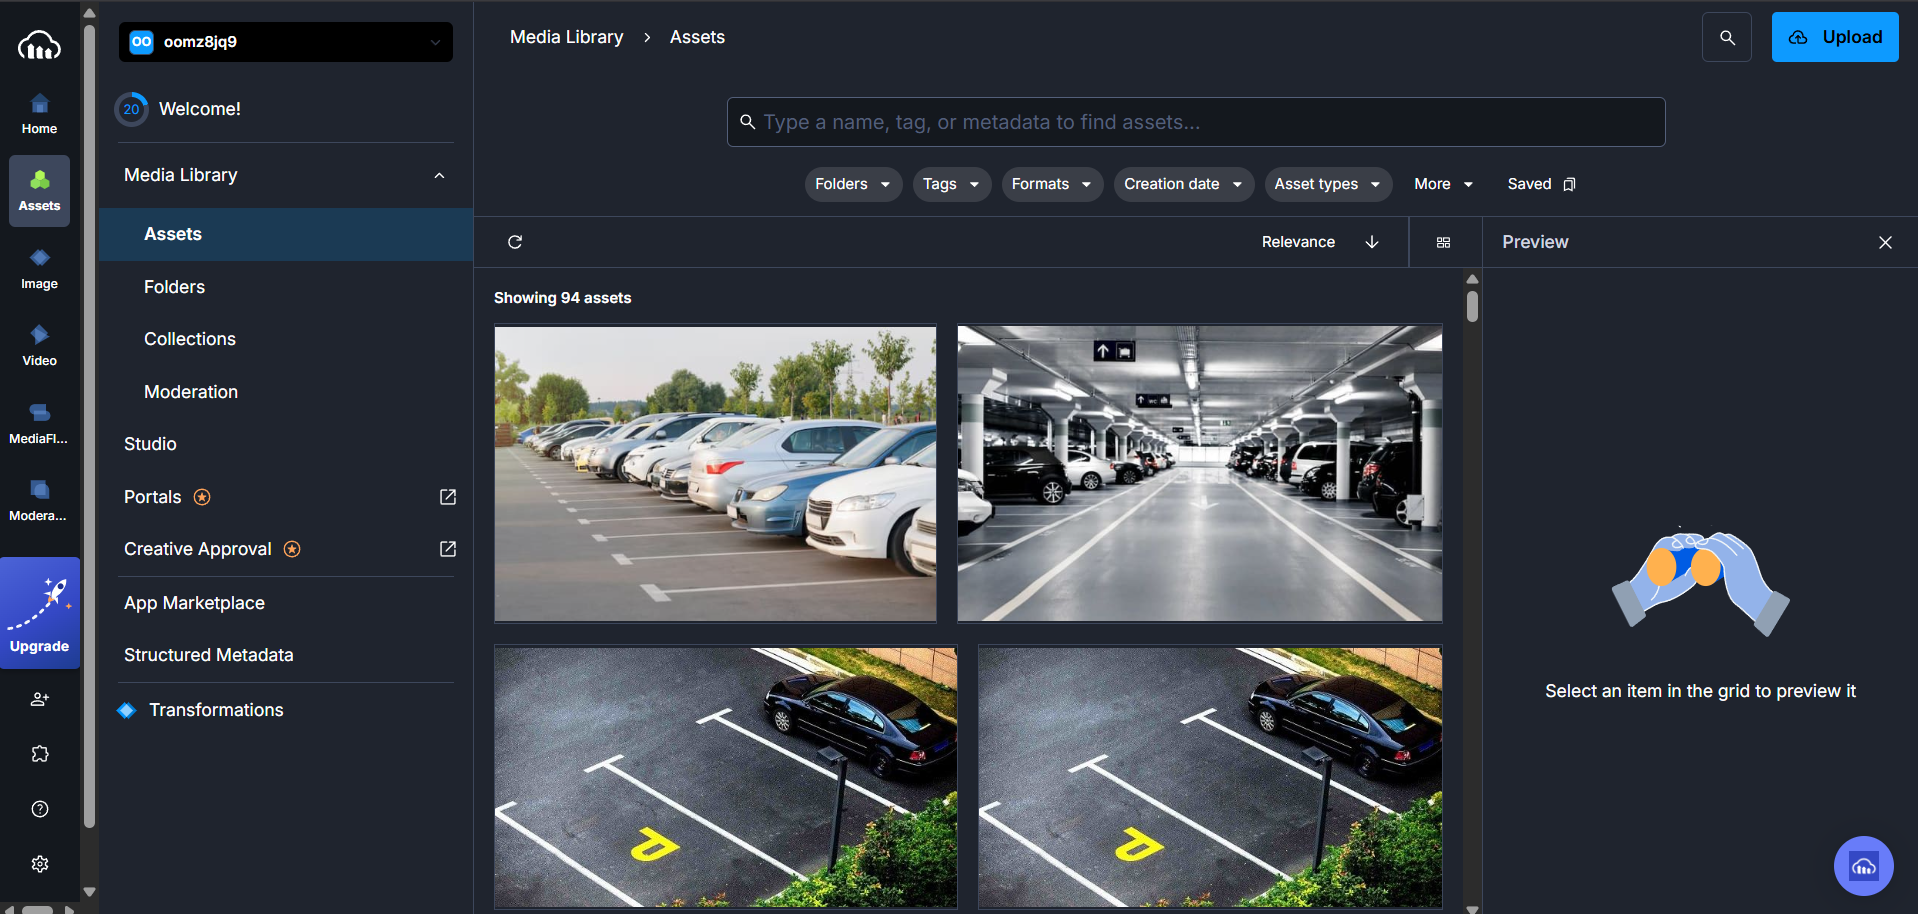
\includegraphics[width=0.9\textwidth]{img/cloudinary_test.png}
    \caption{Validation du stockage des images avec Cloudinary}
    \label{fig:cloudinary_test}
\end{figure}

\par Les essais ont confirmé que les images étaient correctement téléversées, stockées puis affichées dans l'application sans perte de qualité.
\section{Résultats et discussion}

\par Les différentes phases de validation ont confirmé le bon fonctionnement des principales fonctionnalités de l'application \textbf{TuniPark}. Les utilisateurs peuvent créer un compte, s'authentifier de manière sécurisée, consulter les parkings disponibles, démarrer une session de stationnement, effectuer un paiement électronique, recevoir des notifications Push et bénéficier du système de recommandation intelligent. Les propriétaires peuvent proposer leurs parkings privés, tandis que les administrateurs disposent des outils nécessaires pour les valider et assurer la gestion de la plateforme.

\par Les tests ont également permis de vérifier le bon fonctionnement des échanges entre les différents composants de la solution. Le Backend assure la sécurisation des requêtes grâce à l'authentification JWT, communique correctement avec la base de données PostgreSQL et s'intègre aux différents services externes tels que Flouci, Firebase Cloud Messaging et Cloudinary. Le système de recommandation basé sur le modèle Random Forest fournit des recommandations cohérentes en fonction des caractéristiques des parkings et des préférences de l'utilisateur.

\par Malgré les résultats obtenus, certaines améliorations peuvent être envisagées. Parmi celles-ci figurent l'optimisation des performances du système de recommandation à partir d'un plus grand volume de données, l'activation de la vérification des numéros de téléphone par SMS via Twilio, ainsi que l'ajout de nouvelles fonctionnalités de gestion et d'analyse destinées aux administrateurs.

\section{Conclusion}

\par Ce chapitre a présenté les différentes activités de validation réalisées sur l'application \textbf{TuniPark}. Il a couvert les tests des API du Backend, les tests fonctionnels, la validation de la base de données ainsi que la vérification des principaux services externes intégrés à la solution.

\par Les résultats obtenus montrent que les différentes fonctionnalités développées répondent aux exigences définies lors de l'analyse des besoins. Les tests réalisés ont confirmé la fiabilité des principaux modules de l'application, notamment l'authentification, la gestion des parkings, les sessions de stationnement, les paiements électroniques, les notifications Push et le système de recommandation intelligent.

\par Ce travail fournit un socle robuste pour les futures améliorations de l'application. Les améliorations possibles sont exposées dans la conclusion générale de ce travail de recherche.